\chapter{Survey}
\label{survey}

In order to measure if RadGrad has any academic, professional, or social effects on the students, I designed a baseline survey. Unlike the open-ended TechHui data, this survey will ask specific and measurable questions about students' academic, professional, and social experiences in the ICS department, and the results will be used in the future to compare against a similar post-survey. This survey was given to 100 current undergraduate ICS students between January and April 2017. This represents roughly 22\% of the current ICS student population. It was deployed electronically via Google Forms and students completed the survey on an iPad either immediately before or immediately after an advising session with an ICS advisor.  These students are taking advantage of the current department resources available to them, which suggests that they may be the same types of students who would participate in RadGrad. Ultimately, the main goal of the baseline survey is to establish a more specific idea of the state of the ICS undergraduate experience before the integration of RadGrad.

There are three different versions of the survey: prospective students, current students, and graduating students. The prospective students version was given to students who indicated that they were either currently in their first semester of ICS or were planning on taking an ICS course the following semester. The current students version was given to students who indicated that they had completed at least one ICS course and were not planning on graduating within the next year. The graduating students version was given to students who indicated that they were planning on graduating within the next year. Therefore, each baseline survey contains a subset of the following questions. Each question will indicate which group of students were given that question. The full assessment can be found in Appendix \ref{baseline-assessment}. 
\vspace{5mm}
\section{Demographics}

\begin{enumerate}
\begin{figure}[h]
\centering
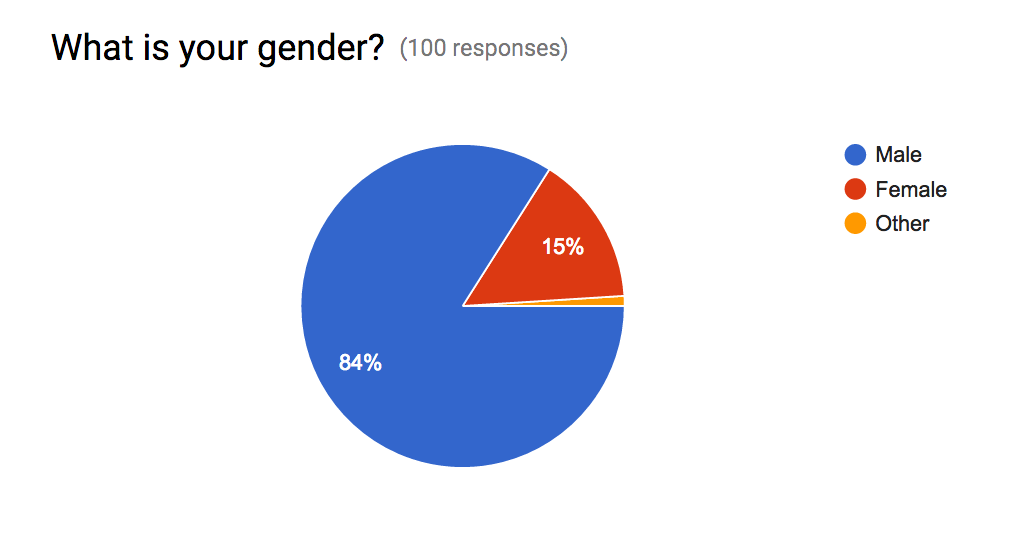
\includegraphics[width=1.0\textwidth]{sr-gender}
\caption{Gender distribution.}
\label{gender}
\end{figure}
\item \textit{What is your gender?}
All participants were given this question (100 total students). In Fall 2016, there was a total of 445 ICS students. Of the 445, 366 identified as male and 79 identified as female (Figure ~\ref{gender}). This means that there was roughly 18\% females and 82\% males. The distribution of my survey has close proportions: 15\% female, 84\% male, and 1\% other. 

\textit{Goals:} This question provides information about the student gender distribution in the ICS department. Since the ICS program currently has significantly more male students than female students, what are are the differences between the experiences of the two genders? Could this give any insight into why there are so little female students? Is this something RadGrad could address? The post survey should investigate if RadGrad has caused any differences in the gender ratio or the disparity between the experiences of the two genders? Ideally, after using RadGrad, both genders should have equally positive experiences in the ICS program.
\begin{figure}[h]
\centering
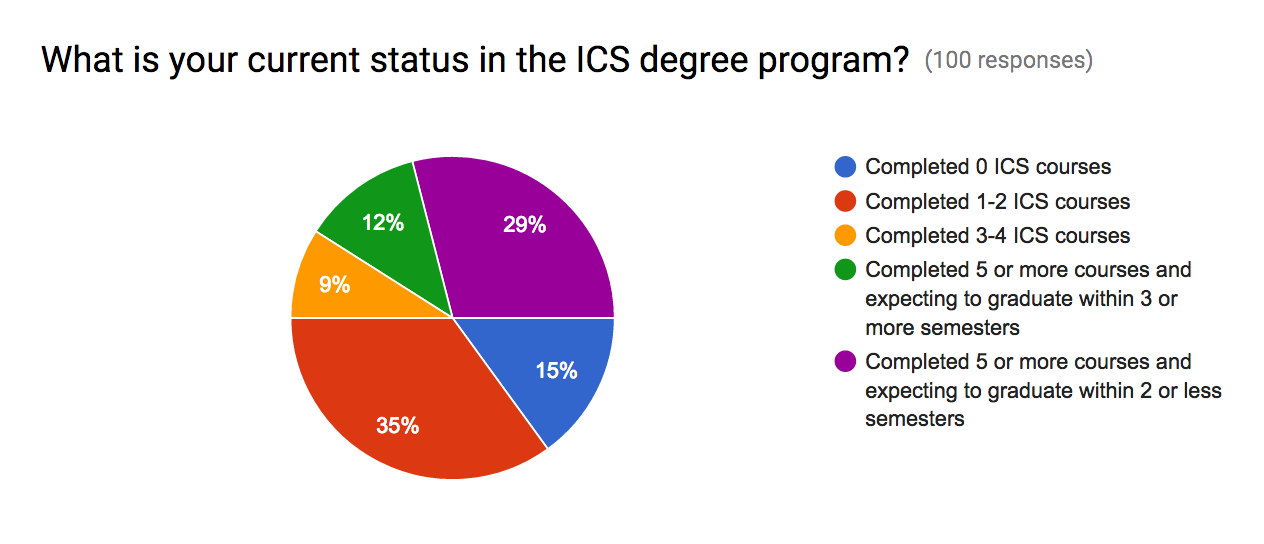
\includegraphics[width=1.0\textwidth]{sr-program-status}
\caption{ICS program status distribution.}
\label{status}
\end{figure}
\item \textit{What is your current status in the ICS degree program?}
All participants were given this question (100 total students). The two most represented groups in the survey are those that had completed 1-2 ICS courses (35\%) and those that had completed 5 or more courses and expected to graduate within 3 or less semesters (29\%) (Figure ~\ref{status}). 15\% of students surveyed were either in or about to start their first semester of ICS. Together, students who were in the middle of the program (completed 3-4 courses or 5 or more courses and expected to graduate within 3 or more semesters) comprised of 21\% of the total population surveyed. The fact that most of the students surveyed were either in the beginning of the program or about to graduate can be attributed to the fact that these are the students that physically go in for advising the most. 

\textit{Goals:} This question provides information that can be used with other questions, to see how student experiences evolve as they progress through the ICS degree program. Are there any patterns? Does RadGrad have any effect on this? The post survey should investigate if RadGrad has certain affects on students in particular stages of the program. Ideally, after using RadGrad, students from all levels should have equally positive experiences in the ICS program. 
\end{enumerate}

\section{Prospective ICS Students}
\begin{enumerate}
\begin{figure}[h]
\centering
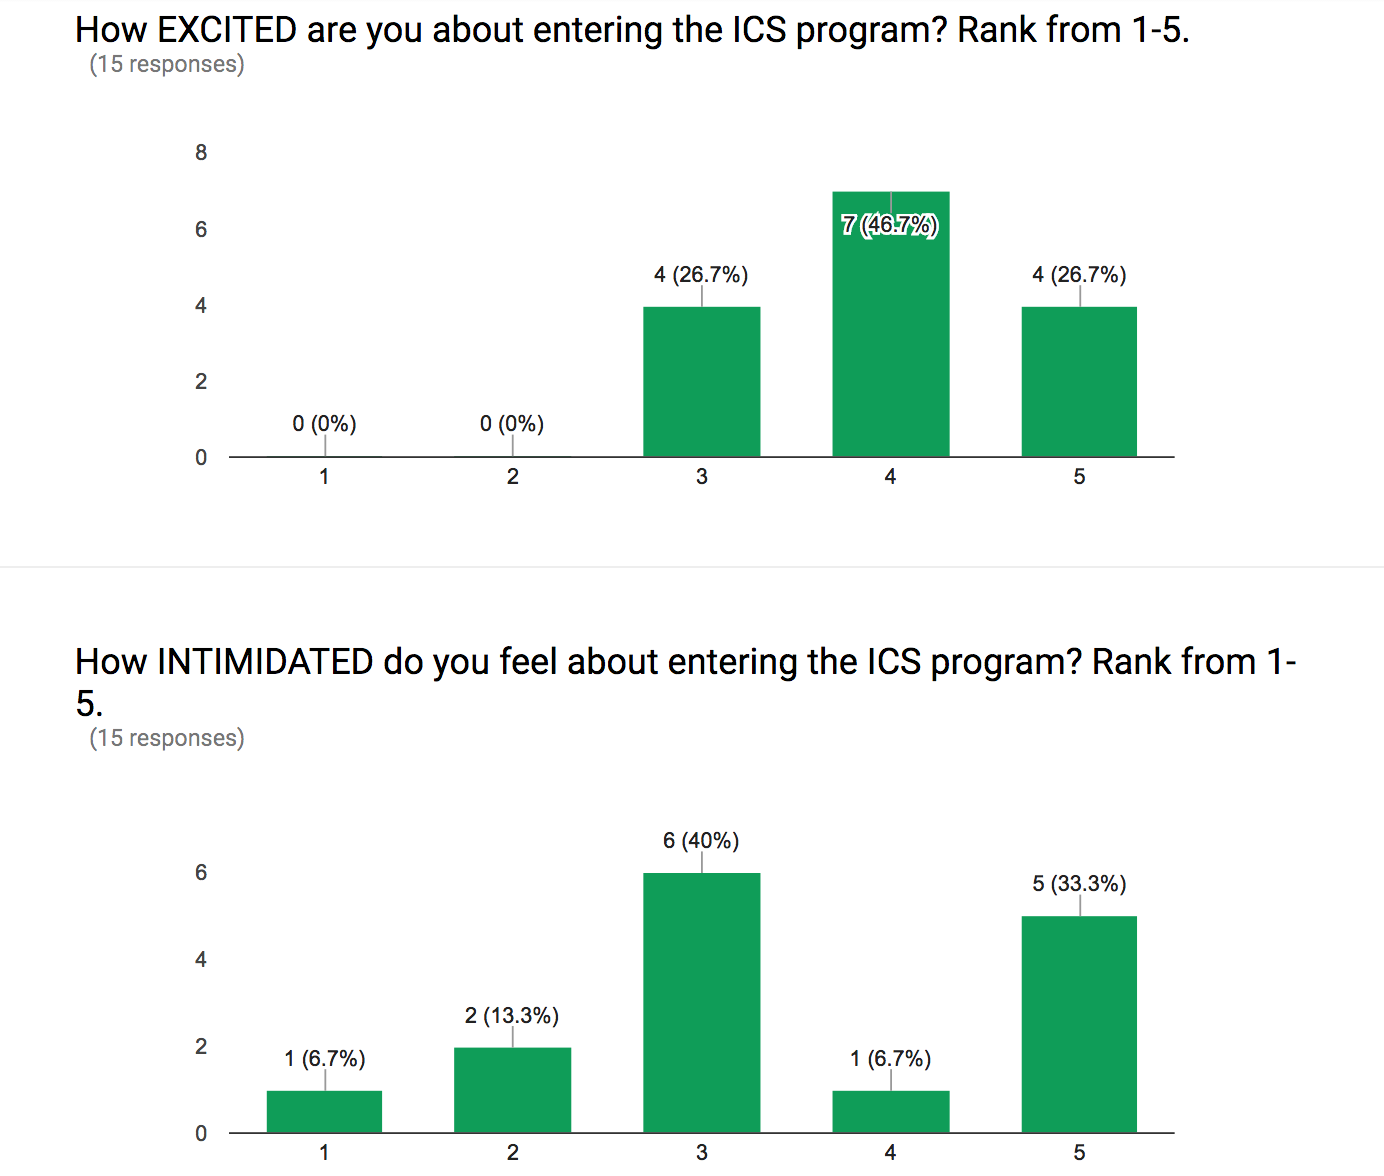
\includegraphics[width=1.0\textwidth]{sr-excited-intimidated}
\caption{Results for prospective ICS Students survey}
\label{excited-intimidated}
\end{figure}
\item\textit{How EXCITED are you about entering the ICS program? Rank from 1-5.}
Only prospective students were given this question (15 total students). The results of the survey show that all of the students surveyed felt either neutral or excited about entering the ICS program (Figure ~\ref{excited-intimidated}). No students stated that they were not excited.

\textit{Goals:} This question will provide information regarding how students view the ICS department, based solely on outside information and their first semester experiences. The post test should investigate the outside factors that affect incoming students' feelings towards the department, and to understand if there are any differences in feelings between genders. Ideally, after using RadGrad, prospective students will feel more excited due to the appearance of a strong, supportive, and diverse community, satisfied alumni, and an appealing program overall. 

\item \textit{How INTIMIDATED do you feel about entering the ICS program? Rank from 1-5.}
Only prospective students were given this question (15 total students). The results of the survey show that a majority of the students surveyed (12 out of 15) felt either neutral or intimidated about entering the ICS program (Figure ~\ref{excited-intimidated}). None of the females surveyed felt less than neutral in regards to intimidation, while three males did feel less than neutral. 

\textit{Goals:} This question will provide information regarding how students view the ICS department, based solely on outside information and their first semester experiences. The post test should investigate the outside factors that affect incoming students' feelings towards the department, and to understand if there are any differences in feelings between genders. Ideally, after using RadGrad, prospective students will feel less intimidated due to the appearance of a strong, supportive, and diverse community, satisfied alumni, and an appealing program overall.

\end{enumerate}

\section{Current ICS Students}
\begin{enumerate}
\begin{figure}[h]
\centering
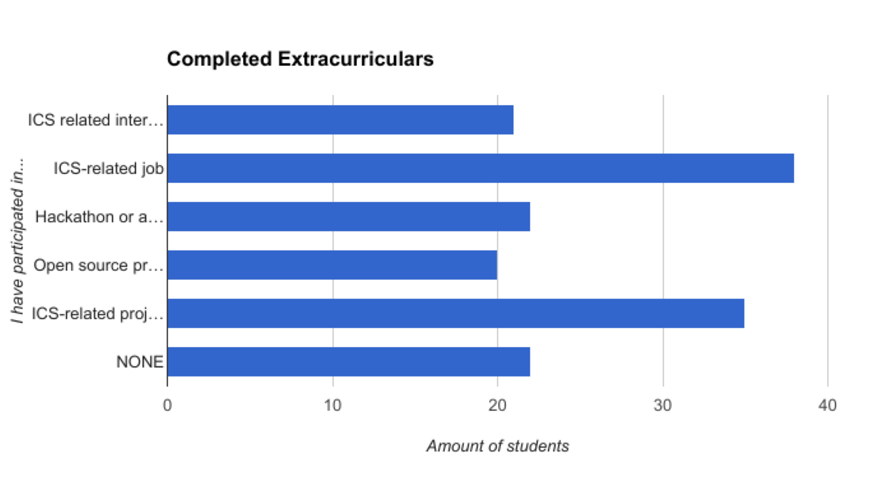
\includegraphics[width=1.0\textwidth]{sr-extracurric-bar}
\caption{Results for extracurricular participation by event type.}
\label{extracurricular}
\end{figure}

\begin{figure}[h]
\centering
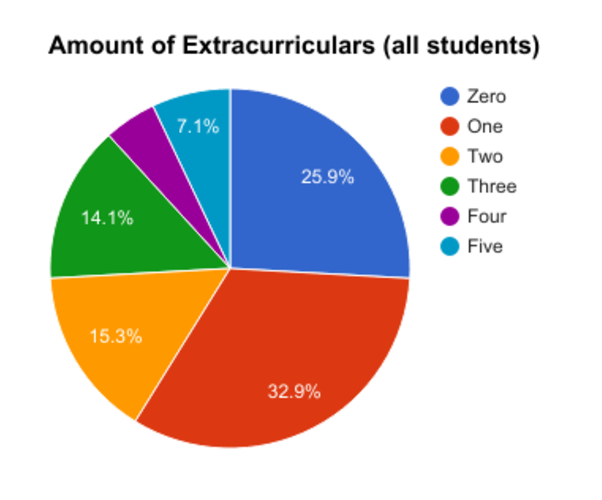
\includegraphics[width=1.0\textwidth]{sr-extracurric-pie}
\caption{Results for extracurricular participation by amount of participation (all students).}
\label{extracurricular-pie-all}
\end{figure}

\begin{figure}[h]
\centering
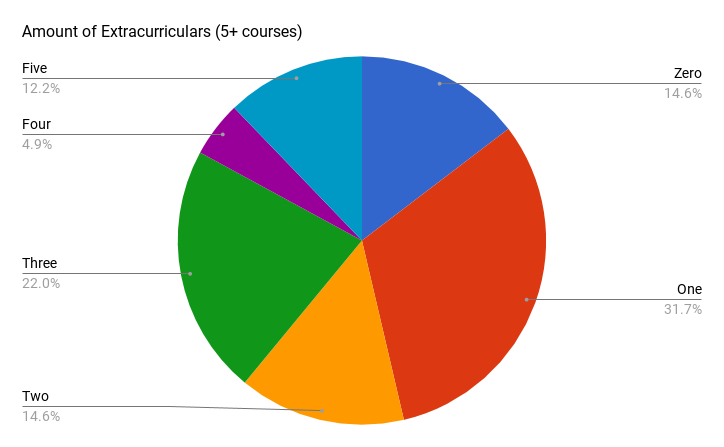
\includegraphics[width=1.0\textwidth]{sr-extracurric-pie-midgrad}
\caption{Results for extracurricular participation by amount of participation (only students who have completed 5+ ICS courses).}
\label{extracurricular-pie-mid-grad}
\end{figure}
\item \textit{Which of the following extracurricular activities, if any, pertain to you?}
Only current and graduating students were given this question (85 total students). Survey results show that out of all the extracurricular activities, the most common was having an ICS related job (38 students), with a close second being doing an ICS-related project outside of class (35 students)(Figure ~\ref{extracurricular}). Participating in an ICS-related internship, hackathon, or open source project each had about 20 students (21, 22, and 20, respectively). Another 22 students hadn't participated in any extracurricular activities. 

Another way to view this data is by the amount of extracurricular participation. In Figure ~\ref{extracurricular-pie-all}, the results show the amount of extracurricular activities that each student participated in. A quarter of students (25.9\%) participated in zero extracurricular activities. About a third of students (32.9\%) participated in just one extracurricular activity. Overall, the data suggests that the amount of extracurricular activities could be negatively correlated to the amount of students participating in them. 
To account for the fact that students in their first year of ICS are at a disadvantage when it comes to extracurricular participation (due to the lack of time and experience), Figure ~\ref{extracurricular-pie-mid-grad} looks at only those students who have completed at least 5 ICS courses. This graph shows that a majority of these students have participated in one extracurricular activity (40.6\%). 21.9\% of students have participated in two extracurricular activities, 15.6\% of students have participated in 0 extracurricular activities, 15.6\% of students have participated in five extracurricular activities, and 6.3\% of students have participated in four extracurricular activities. While this data shows higher levels of participation with mid to graduating students, there are still a significant amount of students who are not participating in any extracurricular activities or participating in only one or two. 

\textit{Goals:} This question provides information about how much initiative students are currently taking to get additional ICS education and experience outside of the classroom. The post survey should investigate if RadGrad can increase the amount and diversity of student involvement in outside ICS-related opportunities due to providing students with stronger connections to the ICS community, and an easier accessibility to these opportunities. Ideally, after using RadGrad, at least 75\% of students who have completed at least 5 ICS courses will have participated in 2 or more extracurricular activities, and close to 0\% of these students will have participated in 0 extracurricular activities. Also, ideally after using RadGrad, students will participate in a wider variety of extracurricular activities.

\begin{figure}[h]
\centering
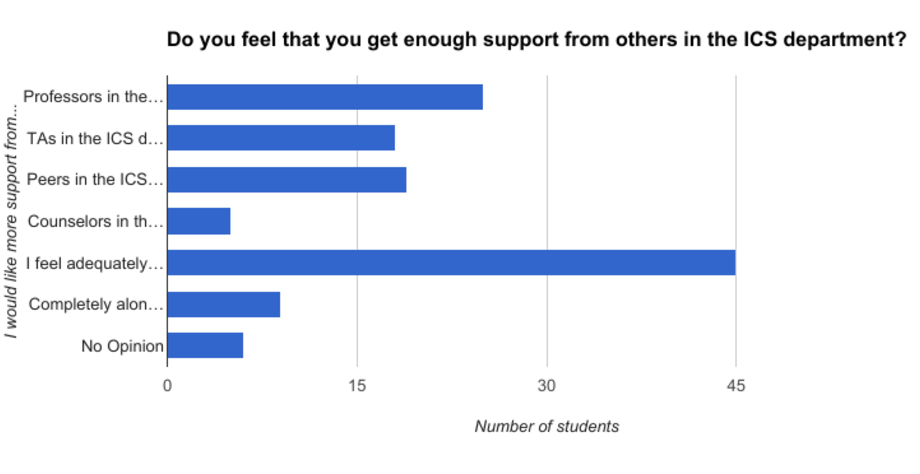
\includegraphics[width=1.0\textwidth]{sr-support-bar}
\caption{Results for support by types of support.}
\label{support-bar}
\end{figure}

\begin{figure}[h]
\centering
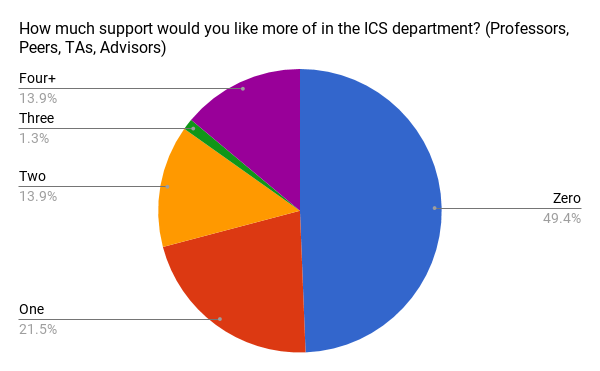
\includegraphics[width=1.0\textwidth]{sr-support-pie}
\caption{Results for support by amount of support desired}
\label{support-pie}
\end{figure}
\item \textit{Do you feel that you get enough support from others in the ICS department?}
Only current and graduating students were given this question (85 total students). Survey results show that a majority of students (45 students) feel adequately supported in the ICS department (Figure ~\ref{support-bar}). However, significant amounts of students desire more support in various areas. 25 students desire more support from professors, 19 students desire more support from their peers, 18 students desire more support from TAs, and 5 students desire more support from advisors. Additionally, 9 students stated that they often feel completely alone in the ICS department and only depend on themselves. 

Another way to view this data is by the extent of the support requested. In Figure ~\ref{support-pie}, the results show the amount of support requested by each student. This graph shows that almost half of the students did not request any further support (49.4\%), while the other half requested further support from at least one group. 21.5\% of students requested further support from one group, 13.9\% requested further support from two groups, 13.9\% requested further support from four or more groups, and 1.3\% requested further support from three groups.  

\textit{Goals:} This question provides information about how satisfied students are with the social aspects of the ICS department. Are students lacking support in certain areas? If so, how can RadGrad help to address these areas? The post survey should investigate exactly how students would like support to be given, and if the social aspects of RadGrad have changed the quality of socialization in the ICS department. Ideally after using RadGrad, at least 50\% of students will feel adequately supported, and close to 0\% of students will feel completely alone within the department.

\begin{figure}[h]
\centering
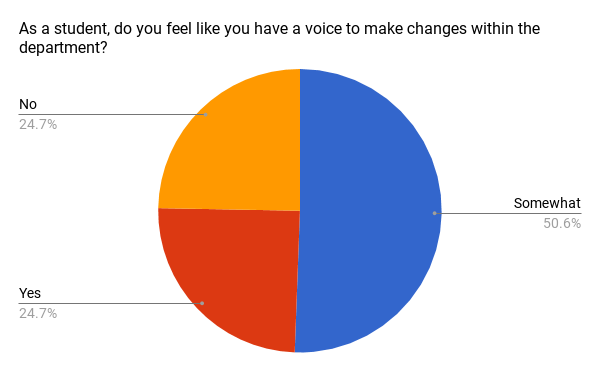
\includegraphics[width=1.0\textwidth]{sr-changes}
\caption{Results for feelings about having a voice to make changes.}
\label{changes}
\end{figure}
\item \textit{As a student, do you feel like you have a voice to make changes within the department?}
Only current and graduating students were given this question (85 total students). Results show that only a quarter of the students surveyed (24.7\%) definitely felt like they have a voice to make changes within the department (Figure ~\ref{changes}). Another quarter (24.7\%) feel like they definitely do not have a voice to make changes, while about half (50.6\%) only somewhat feel like they have a voice to make changes. While the current version of RadGrad does not directly address this issue, it may be addressed in future expansions on RadGrad, such as with the petition feature. 

\textit{Goals:} This question provides information about how much power students feel like they have within the ICS department. What can RadGrad do to help more students feel like they have a voice within the department? The post survey should investigate whether RadGrad has an affect on whether students feel like they have a voice or not. Ideally, after using RadGrad, more than 50\% of the students will feel like they definitely have a voice to make changes within the department.

\begin{figure}[h]
\centering
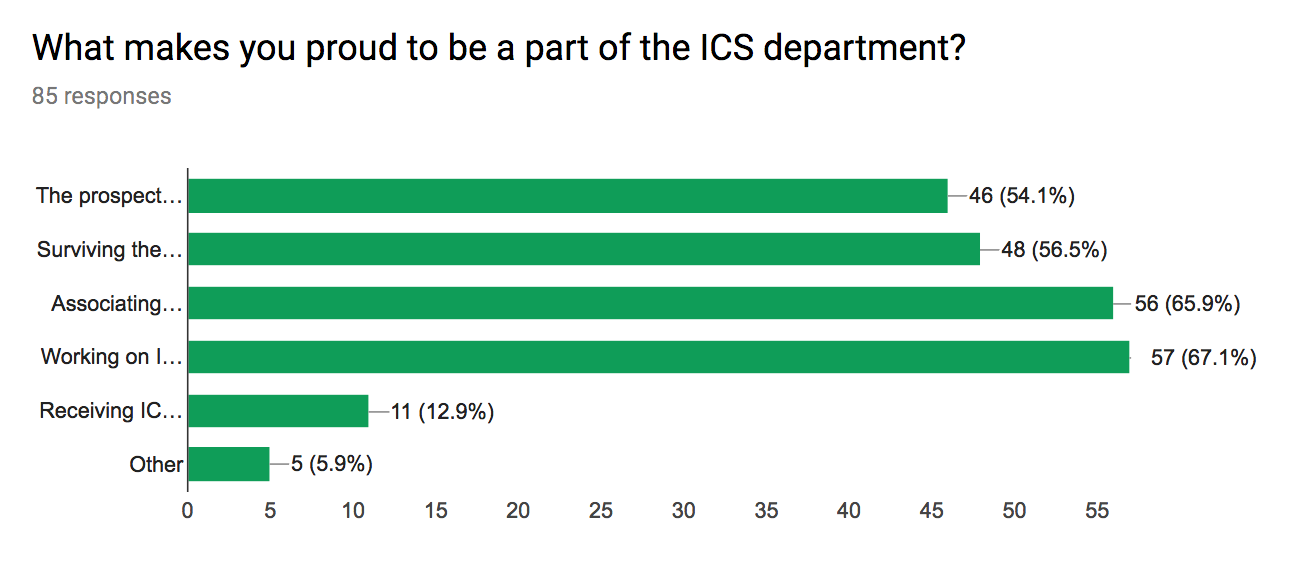
\includegraphics[width=1.0\textwidth]{sr-proud}
\caption{Results for reasons for being proud to be a part of the ICS department.}
\label{proud}
\end{figure}
\item \textit{What makes you proud to be a part of the ICS department?}
Only current and graduating students were given this question (85 total students). Survey results show that a majority of students had at least one reason to feel proud to be a part of the ICS department (Figure ~\ref{proud}). The most popular reasons (in order of decreasing popularity) were working on ICS related projects, associating with the people in ICS, surviving the rigorousness of ICS, and the prospect of finding a high paying job after graduation. The least popular reason, with only 11 students, was receiving ICS awards. Another 5 students chose ``other" without giving a specific reason. 

\textit{Goals:} This question provides information about how current students view the department. A successful department should have a positive reputation among students, which can be manifested with a sense of pride. The post survey should investigate if RadGrad can cause positive changes in the ICS department's reputation, leading to a greater sense of pride among students, which may play a role in students' success. Ideally, after using RadGrad, a majority of students will express their pride for the ICS department in different ways. 

\end{enumerate}

\section{Current ICS Students: Influences}
\begin{enumerate}
\begin{figure}[h]
\centering
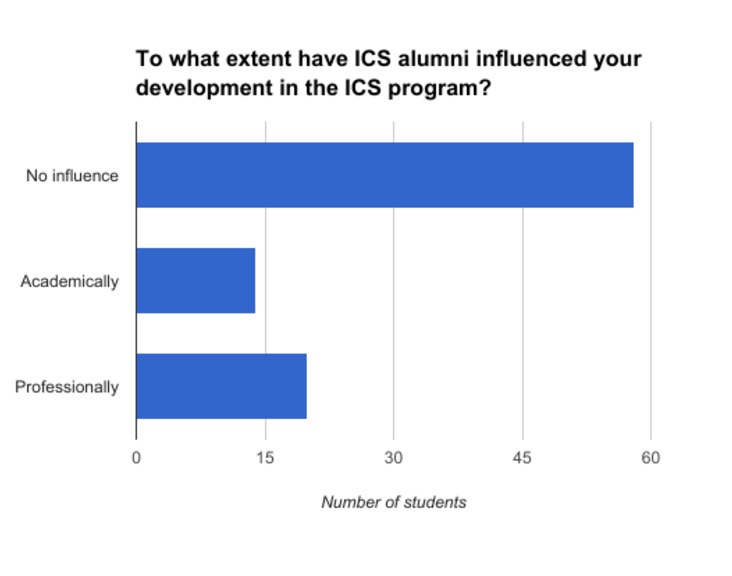
\includegraphics[width=1.0\textwidth]{sr-alumni-influence}
\caption{Results for alumni influence}
\label{alumni-influence}
\end{figure}
\item \textit{To what extent have ICS alumni influenced your development in the ICS program?}
Only current and graduating students were given this question (85 total students). Survey results show that a majority of students (58 our of 84 students) have not been influenced by alumni in any professional or academic way, while 20 out of 84 students have been influenced by an alumni to improve professional development, and 14 out of 84 students have been influenced by an alumni to pursue a major in ICS (Figure ~\ref{alumni-influence}). This suggests that many current ICS students are not interacting with ICS alumni.

\textit{Goals:} This question provides information about the extent of academic and professional interaction between ICS students and alumni. The post survey should investigate if RadGrad adequately provides a way for more students to easily interact with and gain influence from alumni.  Ideally, after using RadGrad, at least 75\% of students will feel like they have been influenced by an alumni in either an academic or professional way. 
   
\begin{figure}[h]
\centering
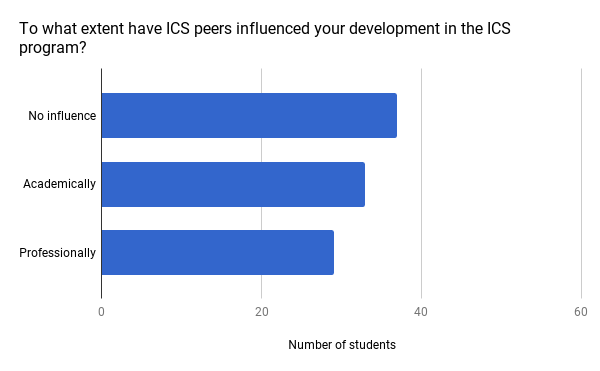
\includegraphics[width=1.0\textwidth]{sr-peer-influence}
\caption{Results for peer influence}
\label{peer-influence}
\end{figure}
\item \textit{To what extent have ICS peers influenced your development in the ICS program?}
Only current and graduating students were given this question (85 total students). Survey results show that a little less than half of students (37 out of 85 students) have not been influenced by their peers in any professional or academic way, while 33 out of 85 students have been influenced by a peer to pursue a major in ICS, and 29 out of 85 students have been influenced by a peer to improve professional development (Figure ~\ref{peer-influence}). This suggests that there is room for improvement when it comes to encouraging academic and professional collaboration among peers. 

\textit{Goals:} This question provides information about the extent of academic and professional interaction between ICS students and their peers. The post survey should investigate if RadGrad adequately provides a way for more students to easily interact with and gain influence from their peers.  Ideally, after using RadGrad, at least 75\% of students will feel like they have been influenced by a peer in either an academic or professional way. 

\begin{figure}[h]
\centering
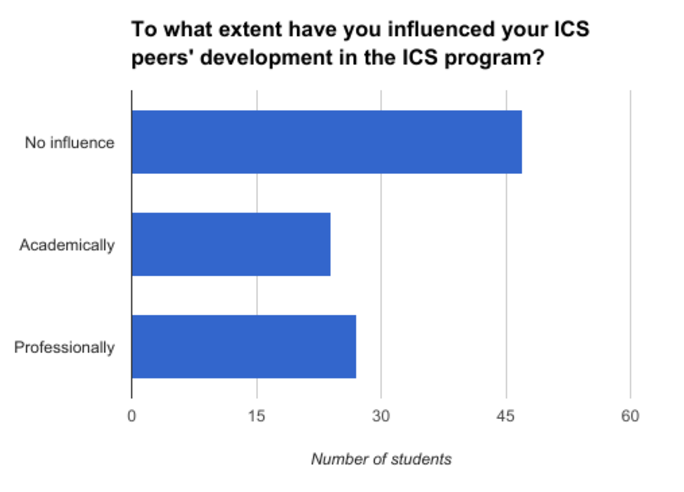
\includegraphics[width=1.0\textwidth]{sr-self-influence}
\caption{Results for student perceptions of their own influence}
\label{self-influence}
\end{figure}
\item \textit{To what extent have you influenced your ICS peers’ development in the ICS program?}
Only current and graduating students were given this question (85 total students). Survey results show that over half of students (49 out of 85 students) feel like they have not influenced their peers in any professional or academic way, while 27 out of 85 students feel like they have influenced a peer to improve professional development, and 25 out of 85 students feel like they have influenced a peer to pursue a major in ICS (Figure ~\ref{self-influence}). This suggests that there is room for improvement when it comes to encouraging academic and professional collaboration among peers.
\textit{Goals:} This question provides information about how students perceive their academic and professional interactions with their peers. The post survey should investigate if RadGrad adequately provides a way for more students to easily interact with and influence their peers.  Ideally, after using RadGrad, at least 75\% of students will feel like they have influenced a peer in either an academic or professional way. 

\end{enumerate}

\section{Graduating ICS Students}
\begin{enumerate}
\begin{figure}[h]
\centering
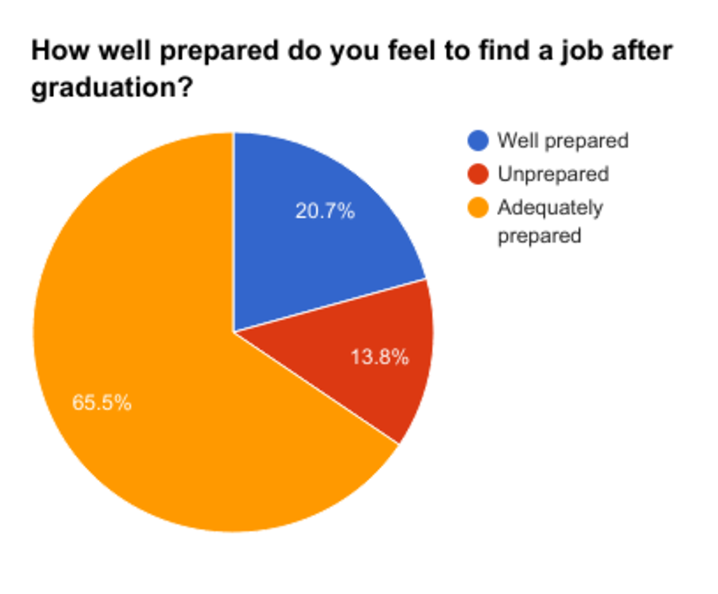
\includegraphics[width=1.0\textwidth]{sr-prepared}
\caption{Results for graduation preparedness.}
\label{prepared-grad}
\end{figure}
\item \textit{Now that you are nearing the end of your ICS degree program experience, how well prepared do you feel to find a job after graduation?}
Only graduating students were given this question (29 total students). Survey results show that only 20.7\% of graduating students feel well prepared to find a job after graduation (Figure ~\ref{prepared-grad}). 65.5\% of graduating students feel adequately prepared, and 13.8\% of students feel unprepared. This suggests that there is room for improvement when it comes to preparing students for the workforce in a way that makes them feel more confident and prepared. 

\textit{Goals:} This question provides information about the amounts of students that feel well prepared. What can RadGrad do to help more students feel well prepared to find a job after graduation? The post survey should test to see if RadGrad's encouragement of collaboration and a well-balanced education (with both courses and opportunities) causes more students to feel well prepared to find a job after graduation. Ideally, after using RadGrad, more than half of graduating students will feel well prepared for the future.

\begin{figure}[h]
\centering
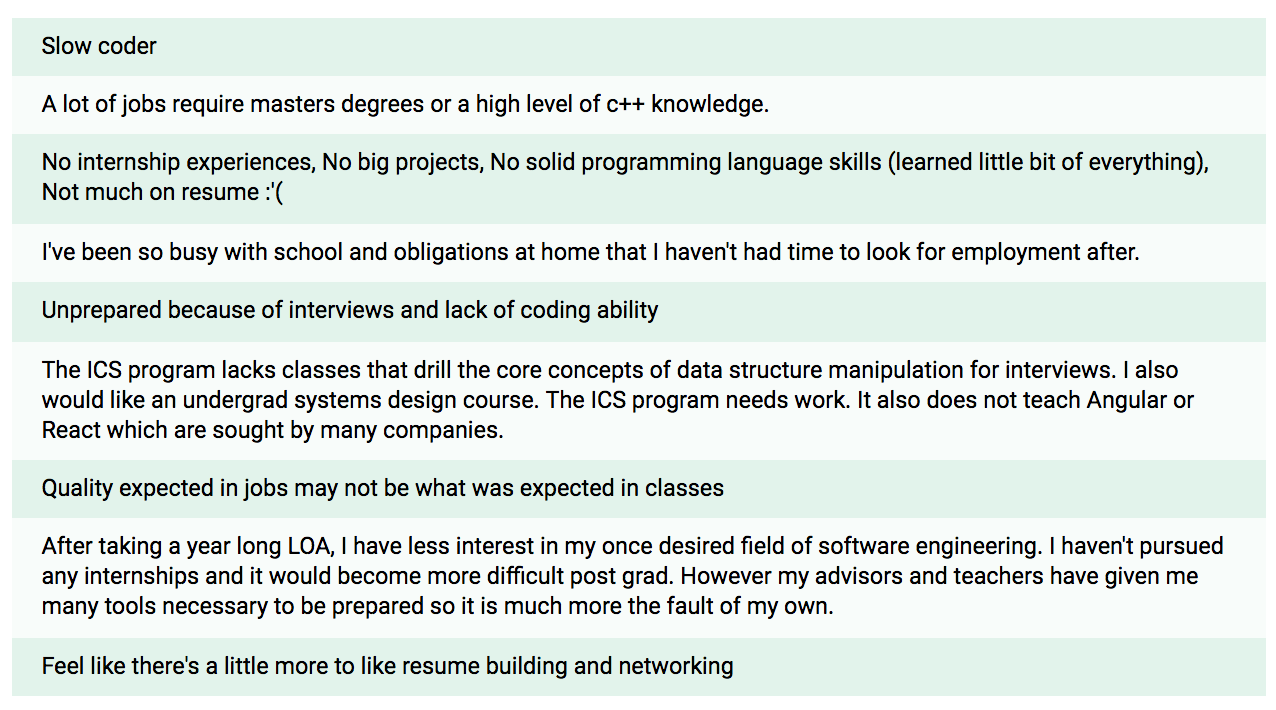
\includegraphics[width=1.0\textwidth]{sr-unprepared-grad-reasons}
\caption{Reasons for not feeling prepared for graduation.}
\label{reasons}
\end{figure}
\item \textit{If you answered above that you feel unprepared to find a job after graduation, please explain why. }
Only graduating students were given this question (29 total students). Figure ~\ref{reasons} lists reasons that students have for not feeling well prepared to find a job after graduation. These reasons suggest that RadGrad could have a positive impact by encouraging students to pursue ICS related experiences outside of the classroom.

\textit{Goals:} This question provides information about problems or regrets that students realize right before they graduate. Are there any common reasons for students not feeling prepared? If so, is there anything RadGrad can do to address these problems? The post survey should reveal whether there has been any changes in the reasons given for students not feeling well prepared. Ideally, after using RadGrad, the reasons given for not feeling well prepared will no longer focus on the lack of outside experience. 

\end{enumerate}

Ideally, after RadGrad, future studies will show that there is less disparity between student expectations and reality, greater student satisfaction with the department, more student engagement, and more positive student feelings overall.


